\documentclass{JINST}
\usepackage{cite}
\newcommand{\li}{$^{9}$Li~}
\newcommand{\he}{$^{8}$He~}
\newcommand{\beEIGHT}{$^{8}$Be~}
\newcommand{\beNINE}{$^{9}$Be~}
\newcommand{\heFIVE}{$^{5}$He~}

\title{A nuclear physics-based Monte Carlo of the \li  and \he  comsogenic production in liquid scintillator experiments.}

\author{First Author$^a$, Second Author$^b$\thanks{Corresponding
author.}~ and Third Author$^b$\\
\llap{$^a$}Name of Institute,\\
  Address, Country\\
\llap{$^b$}Name of Institute,\\
  Address, Country\\
  E-mail: \email{CorrespondingAuthor@email.com}}


\abstract{Radioactive isotopes that decay into beta and a delayed neutron pair are considered a signficant background to liquid scintilator based neutrino experiments since
they mimic the anti-neutrino signature in the detector. Lithium-9 and Helium-8 are some of such isotopes. 
While estimating the (the absolute yield of the isotope) rate of such isotopes poses a challenge, the simulation of the decay spectrum  of such isotopes 
is feasable. In this work we present a Monte Carlo simulations of the \li/\he decay spectra accomplished using
a literature review of decay properties of the different decay branches of such isotopes. While the applicability of the 
generator presented here is generic to other experiments as well, the generator output
is specifically compared to the output simulations of the Double Chooz reactor experiment.}


\keywords{Keyword1; Keyword2; Keyword3}

\begin{document}

\section{Introduction}


      Many neutrino experiments have published results of cosmogenic background measurements needed for
      the precise predictions of neutrino oscilations. Of such experiments, the neutrino experiment 
      KamLAND has published an extensive comparison of the cosmogenics measurements with 
      predictions based on Monte Carlo simulations ~\cite{PhysRevC.81.025807}. The predictions published show an excellent agreement
      with the experimental measurements.
     
     
     Measurements and predictions of the cosmogenics (of special interest here \li and \he) are necessary since they
      have the following signature; beta decay followed by a delayed neutron that gets captured on the 
      target scintillator. Such a reaction is similar to the inverse beta decay reaction:

      \mbox{$\bar{\nu}_e + p \rightarrow e^+ + n$}
      
      
      used in liquid scintillator experiments to detect incoming anti-neutrinos (apart from the inability for the 
      currently built liquid scintillator detectors to distinguish negative beta (electrons) from positive beta decays (positrons)).


      This paper is organized as follows; section~\ref{section1} discusses a brief overview of
      how the generator works. Followed by section~\ref{section2} where a discussion of the 
      results of the generator is done. And finally section~\ref{section3} summarizes with a conclusion.
      

\section{The Cosmogenics Generator}
\label{section1}

The generator used in this work was constructed by incorporating all the decay properties of 
the different possible decay states of the cosmogenic isotope in interest (\li or \he). Such properties include;
energy of the decaying state (and uncertainties associated with it),
the branching ratio of the state (and uncertainties associated with it)............

The current state of the generator involves the construction of the different 
 probabilities for the isotopes decay. The output of the generator is a list 
 of either; beta, neutron or alpha particles. Each of the emitted particles carry momentum 
 according to a simplified momentum-splitting formula;
 
 
 
 \begin{equation}
K_1 = E \frac{m}{M}
\end{equation}
and 
\begin{equation}
K_2 = E \frac{M-m}{M}
\end{equation}


where $m$ is the mass of one of the daughters and $M$ is the decaying mass. 
 

\subsection{The \li decay scheme}
 In fig.~\ref{DecayScheme} the Li9 decay states relevant to the 
 liquid scintilator experiments are shown.
 
 \begin{figure}
  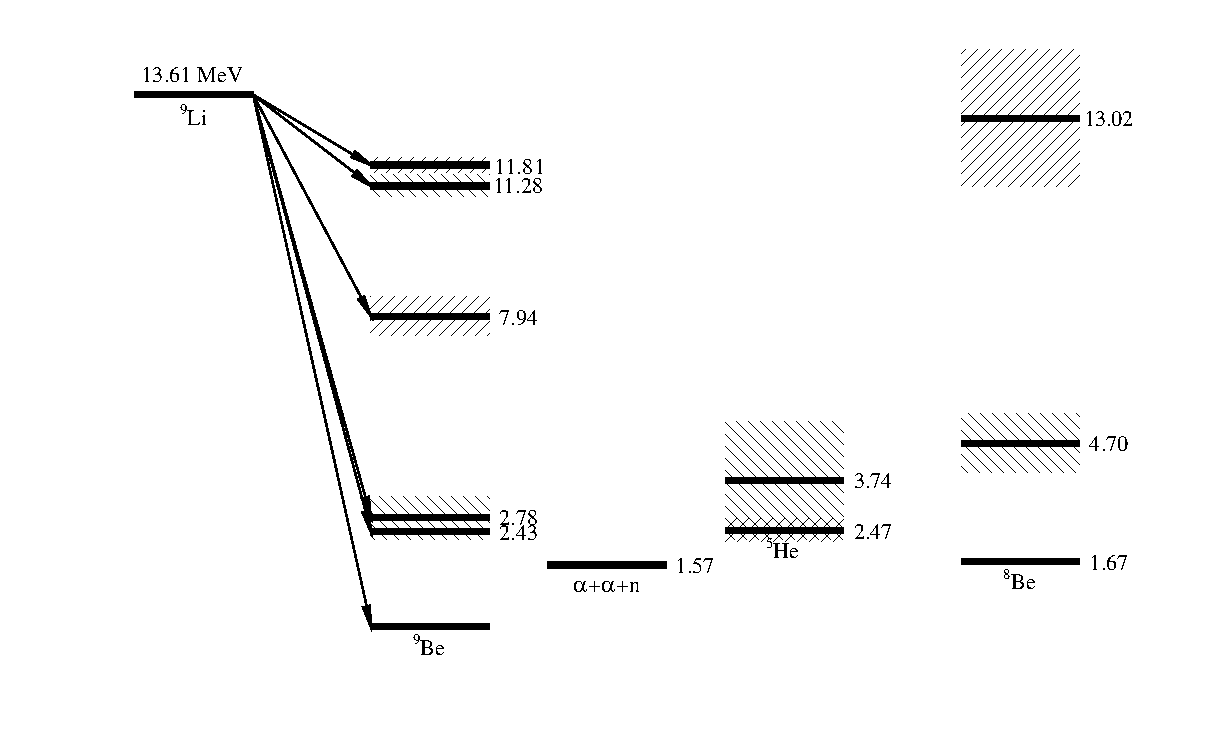
\includegraphics[width=100mm]{Lithium9DecayScheme.eps}
  \label{DecayScheme}
  \caption{A schematic of the \li decay scheme. }
 \end{figure}
 
 The energy states of the decay products relevant to this study are :
 
\begin{table}
\caption{\label{tab:statesH1} {\bf The \beNINE state}: energy states, branching ratios and their associated uncertainties.~\cite{Prezado200355}.}
\begin{center}
\begin{small}
\begin{tabular}{l l l l l}
\hline
Sub-branch & BR & \delta BR & $E$ & $\delta E$ \\
\hline
1. $^{5}$He(g.s.) + $\alpha$ & 0.28 & $\pm$0.06 & 2.467 & $\pm$0.648 \\ 
2. $^{5}$He(1/2-) + $\alpha$ & 0.47 & $\pm$0.07 & 3.737 & $\pm$5.57 \\
3. $^{8}$Be(g.s.) + n & 0.02 & $\pm$0.01 & 1.6654 & $\pm$0.00557 \\
4. $^{8}$Be(2+) + n  & 0.11 & $\pm$0.06 & 4.695 & $\pm$1.513 \\
5. $^{8}$Be(4+) + n & 0.12 & $\pm$0.08  &  13.015 & $\pm$3.500 \\
\hline
\end{tabular}
\end{small}
\end{center}
\end{table}




\begin{table}
\caption{\label{tab:statesH2} The kinetic energy of particles from the various break-up scenarios of 11.81~MeV state of $^{9}$Be. Units are in keV and the branching fraction is from Ref.~\cite{Prezado200355}.}
\begin{center}
\begin{small}
\begin{tabular}{l l l l l}
\hline
Sub-branch & BR & \delta BR & $E$ & $\delta E$ \\
\hline
1. $^{5}$He(g.s.) + $\alpha$ & 0.28 & $\pm$0.06 & 560.6 & 2242.6 \\ 
2. $^{5}$He(1/2-) + $\alpha$ & 0.47 & $\pm$0.07 & 639.0 & 2556.2 \\
3. $^{8}$Be(g.s.) + n & 0.02 & $\pm$0.01 & 541.8 & 9017.4 \\
4. $^{8}$Be(2+) + n  & 0.11 & $\pm$0.06 & 1738.8 & 6324.1 \\
5. $^{8}$Be(4+) + n & 0.12 & $\pm$0.08  &  5085.2 & 0.1 \\
\hline
\end{tabular}
\end{small}
\end{center}
\end{table}



 \begin{table}
\caption{\label{tab:statesH3} {\bf The \beNINE state}: energy states, branching ratios and their associated uncertainties.~\cite{Prezado200355}.}
\begin{center}
\begin{small}
\begin{tabular}{l l l l l}
\hline
Sub-branch & BR & \delta BR & $E$ & $\delta E$ \\
\hline
1. $^{5}$He(g.s.) + $\alpha$ & 0.28 & $\pm$0.06 & 2.467 & $\pm$0.648 \\ 
2. $^{5}$He(1/2-) + $\alpha$ & 0.47 & $\pm$0.07 & 3.737 & $\pm$5.57 \\
3. $^{8}$Be(g.s.) + n & 0.02 & $\pm$0.01 & 1.6654 & $\pm$0.00557 \\
4. $^{8}$Be(2+) + n  & 0.11 & $\pm$0.06 & 4.695 & $\pm$1.513 \\
5. $^{8}$Be(4+) + n & 0.12 & $\pm$0.08  &  13.015 & $\pm$3.500 \\
\hline
\end{tabular}
\end{small}
\end{center}
\end{table}




\begin{table}
\caption{\label{tab:statesH4} {\bf The \beNINE state}: energy states, branching ratios and their associated uncertainties.~\cite{Prezado200355}.}
\begin{center}
\begin{small}
\begin{tabular}{l l l l l}
\hline
Sub-branch & BR & \delta BR & $E$ & $\delta E$ \\
\hline
1. $^{5}$He(g.s.) + $\alpha$ & 0.28 & $\pm$0.06 & 2.467 & $\pm$0.648 \\ 
2. $^{5}$He(1/2-) + $\alpha$ & 0.47 & $\pm$0.07 & 3.737 & $\pm$5.57 \\
3. $^{8}$Be(g.s.) + n & 0.02 & $\pm$0.01 & 1.6654 & $\pm$0.00557 \\
4. $^{8}$Be(2+) + n  & 0.11 & $\pm$0.06 & 4.695 & $\pm$1.513 \\
5. $^{8}$Be(4+) + n & 0.12 & $\pm$0.08  &  13.015 & $\pm$3.500 \\
\hline
\end{tabular}
\end{small}
\end{center}
\end{table}




\begin{table}
\caption{\label{tab:statesH5} {\bf The \beNINE state}: energy states, branching ratios and their associated uncertainties.~\cite{Prezado200355}.}
\begin{center}
\begin{small}
\begin{tabular}{l l l l l}
\hline
Sub-branch & BR & \delta BR & $E$ & $\delta E$ \\
\hline
1. $^{5}$He(g.s.) + $\alpha$ & 0.28 & $\pm$0.06 & 2.467 & $\pm$0.648 \\ 
2. $^{5}$He(1/2-) + $\alpha$ & 0.47 & $\pm$0.07 & 3.737 & $\pm$5.57 \\
3. $^{8}$Be(g.s.) + n & 0.02 & $\pm$0.01 & 1.6654 & $\pm$0.00557 \\
4. $^{8}$Be(2+) + n  & 0.11 & $\pm$0.06 & 4.695 & $\pm$1.513 \\
5. $^{8}$Be(4+) + n & 0.12 & $\pm$0.08  &  13.015 & $\pm$3.500 \\
\hline
\end{tabular}
\end{small}
\end{center}
\end{table}





\begin{table}
\caption{\label{tab:statesH6} {\bf The \beNINE state}: energy states, branching ratios and their associated uncertainties.~\cite{Prezado200355}.}
\begin{center}
\begin{small}
\begin{tabular}{l l l l l}
\hline
Sub-branch & BR & \delta BR & $E$ & $\delta E$ \\
\hline
1. $^{5}$He(g.s.) + $\alpha$ & 0.28 & $\pm$0.06 & 2.467 & $\pm$0.648 \\ 
2. $^{5}$He(1/2-) + $\alpha$ & 0.47 & $\pm$0.07 & 3.737 & $\pm$5.57 \\
3. $^{8}$Be(g.s.) + n & 0.02 & $\pm$0.01 & 1.6654 & $\pm$0.00557 \\
4. $^{8}$Be(2+) + n  & 0.11 & $\pm$0.06 & 4.695 & $\pm$1.513 \\
5. $^{8}$Be(4+) + n & 0.12 & $\pm$0.08  &  13.015 & $\pm$3.500 \\
\hline
\end{tabular}
\end{small}
\end{center}
\end{table}






 \section{Monte Carlo Results}
\label{section2} 
 In this section we present the results obtained with the generator.
 

 The Monte Carlo simulations used by the Double Chooz collaboration is based on 
 a GEANT4 (version) ~\cite{} simulation of the Double Chooz detector and the generic liquid scintillator
 neutrino experiment package GLG4sim ~\cite{}. The results obtained by running the generator 
 independently of the Double Chooz detector simulations is refered to as \textbf{{\emph{particle level}}}, while 
 results obtained by running the generator output through the simulations of the Double Chooz detector 
 are refered to as  \textbf{{\emph{detector level}}}.
\subsection{Paricle Level}


%\begin{figure}
%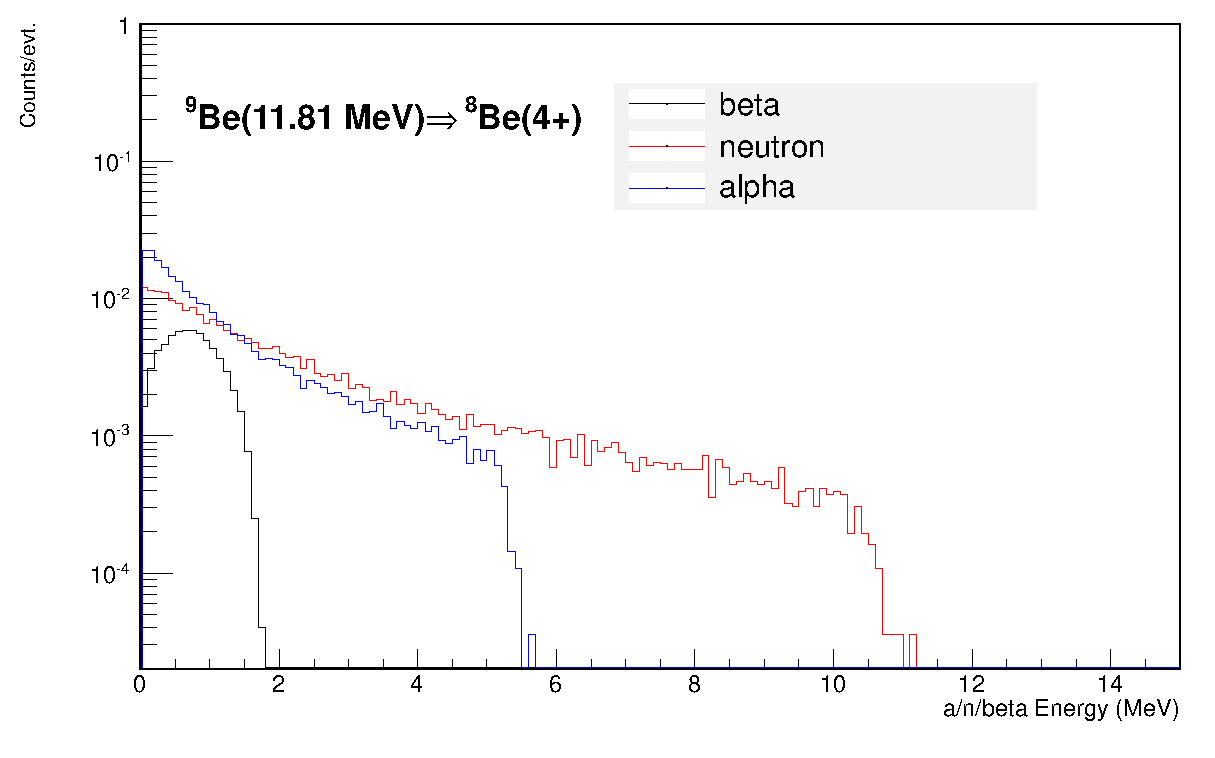
\includegraphics[scale=0.45]{a_n_beta_spect_c20.eps}
%\caption{
%Average target detector response evolution in time, as 
%measured by the mean energy of the Gd-capture peak arising from 
%interaction of spallation neutrons in the NT.
%\label{fig:gstability}}
%\end{figure}

\begin{figure}[htp]

  \centering

  

  \begin{tabular}{cc}

    % Requires \usepackage{graphicx}

    \includegraphics[width=60mm]{a_n_beta_spect_c2.eps}&

    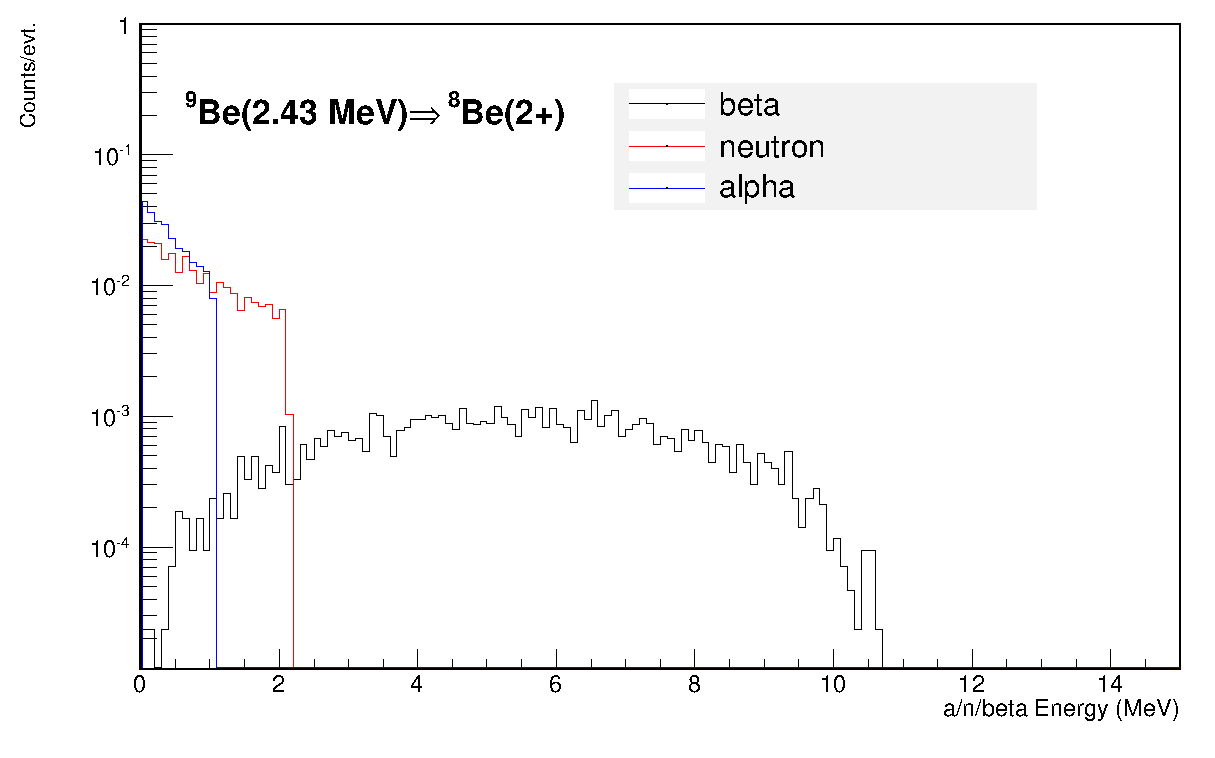
\includegraphics[width=60mm]{a_n_beta_spect_c3.eps}\\

    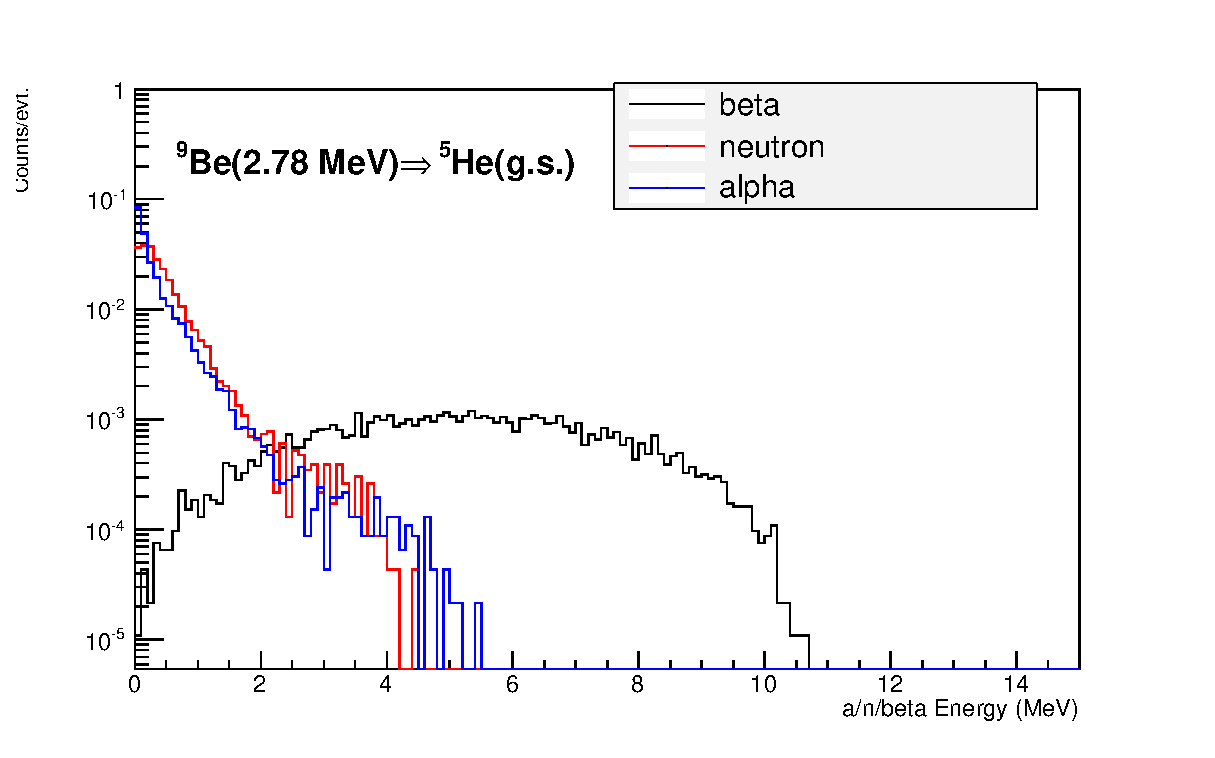
\includegraphics[width=60mm]{a_n_beta_spect_c4.eps}&

    \includegraphics[width=60mm]{a_n_beta_spect_c5.eps}\\

      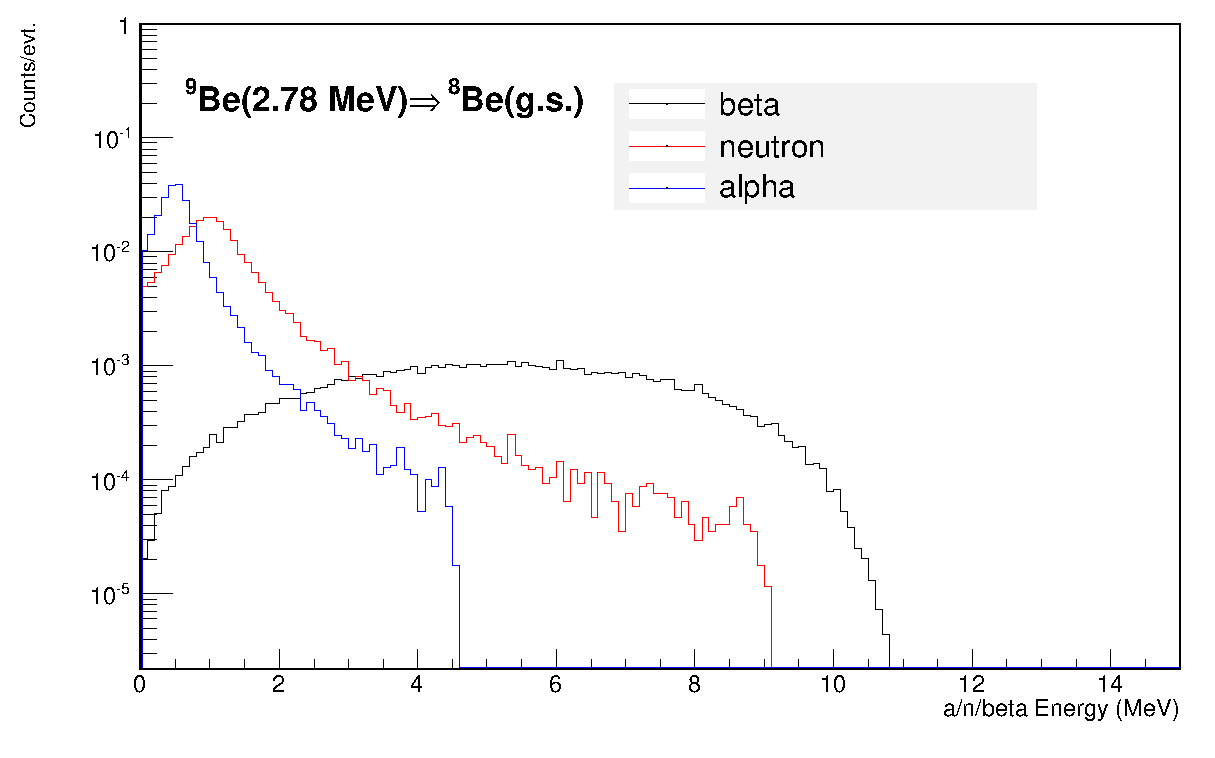
\includegraphics[width=60mm]{a_n_beta_spect_c6.eps}&

    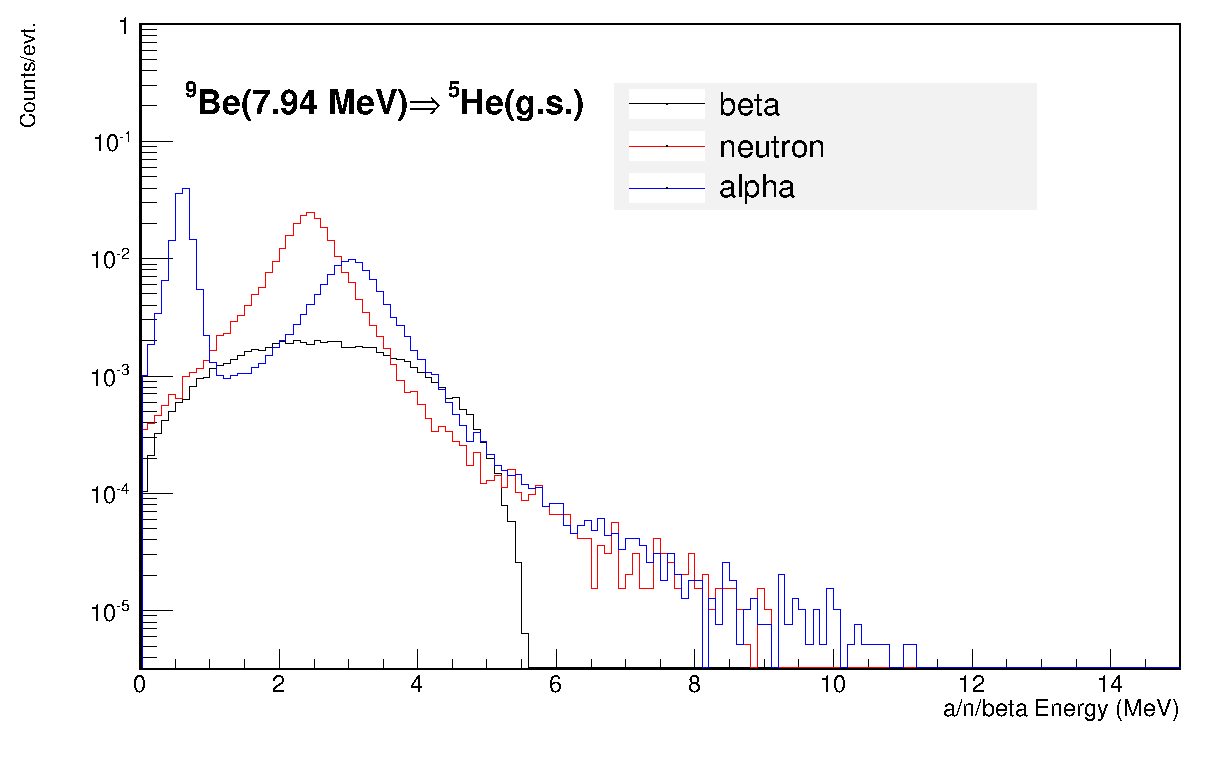
\includegraphics[width=60mm]{a_n_beta_spect_c7.eps}\\
   
  \end{tabular}
\label{figur}\caption{ Particle level energy distributions.}
\end{figure}
        Tasdfah asoiuh siuhihosi soiu hskjd asoiuh siuhihosi soiu
hskjd. Asoiuh siuhihosi soiu hskjd asoiuh siuhihosi soiu hskjd. Asoiuh
siuhihosi soiu hskjd asoiuh siuhihosi soiu hskjd.  Asoiuh siuhihosi
soiu hskjd asoiuh siuhihosi soiu hskjd. Asoiuh siuhihosi soiu hskjd
asoiuh siuhihosi soiu hskjd. Asoiuh siuhihosi soiu hskjd asoiuh
siuhihosi soiu hskjd. Asoiuh siuhihosi soiu hskjd asoiuh siuhihosi
soiu hskjd. Asoiuh siuhihosi soiu hskjd asoiuh siuhihosi soiu hskjd.
Asoiuh siuhihosi soiu hskjd asoiuh siuhihosi soiu hskjd. Asoiuh
siuhihosi soiu hskjd asoiuh siuhihosi soiu hskjd. Asoiuh siuhihosi
soiu hskjd asoiuh siuhihosi soiu hskjd. Asoiuh siuhihosi soiu hskjd
asoiuh siuhihosi soiu hskjd. Asoiuh siuhihosi soiu hskjd asoiuh
siuhihosi soiu hskjd.  Asoiuh siuhihosi soiu hskjd asoiuh siuhihosi
soiu hskjd. Asoiuh siuhihosi soiu hskjd asoiuh siuhihosi soiu
hskjd. Asoiuh siuhihosi soiu hskjd asoiuh siuhihosi soiu hskjd. Asoiuh
siuhihosi soiu hskjd asoiuh siuhihosi soiu hskjd.


%\subsubsection{Subsubsection}

        Tasdfah asoiuh siuhihosi soiu hskjd asoiuh siuhihosi soiu
hskjd. Asoiuh siuhihosi soiu hskjd asoiuh siuhihosi soiu hskjd. Asoiuh
siuhihosi soiu hskjd asoiuh siuhihosi soiu hskjd.  Asoiuh siuhihosi
soiu hskjd asoiuh siuhihosi soiu hskjd. Asoiuh siuhihosi soiu hskjd
asoiuh siuhihosi soiu hskjd. Asoiuh siuhihosi soiu hskjd asoiuh
siuhihosi soiu hskjd. Asoiuh siuhihosi soiu hskjd asoiuh siuhihosi
soiu hskjd. Asoiuh siuhihosi soiu hskjd asoiuh siuhihosi soiu hskjd.
Asoiuh siuhihosi soiu hskjd asoiuh siuhihosi soiu hskjd. Asoiuh
siuhihosi soiu hskjd asoiuh siuhihosi soiu hskjd. Asoiuh siuhihosi
soiu hskjd asoiuh siuhihosi soiu hskjd. Asoiuh siuhihosi soiu hskjd
asoiuh siuhihosi soiu hskjd. Asoiuh siuhihosi soiu hskjd asoiuh
siuhihosi soiu hskjd. 


\subsection{Detector Level}

        Tasdfah asoiuh siuhihosi soiu hskjd asoiuh siuhihosi soiu
hskjd. Asoiuh siuhihosi soiu hskjd asoiuh siuhihosi soiu hskjd. Asoiuh
siuhihosi soiu hskjd asoiuh siuhihosi soiu hskjd.  Asoiuh siuhihosi
soiu hskjd asoiuh siuhihosi soiu hskjd. Asoiuh siuhihosi soiu hskjd
asoiuh siuhihosi soiu hskjd.

Asoiuh siuhihosi soiu hskjd asoiuh siuhihosi soiu hskjd.  Asoiuh
siuhihosi soiu hskjd asoiuh siuhihosi soiu hskjd. Asoiuh siuhihosi
soiu hskjd asoiuh siuhihosi soiu hskjd. Asoiuh siuhihosi soiu hskjd
asoiuh siuhihosi soiu hskjd. Asoiuh siuhihosi soiu hskjd asoiuh
siuhihosi soiu hskjd. Asoiuh siuhihosi soiu hskjd asoiuh siuhihosi
soiu hskjd. Asoiuh siuhihosi soiu hskjd asoiuh siuhihosi soiu hskjd.

\begin{figure}[htp]

  \centering

  

  \begin{tabular}{cc}

    % Requires \usepackage{graphicx}

    \includegraphics[width=60mm]{MC_Li_10.eps}&

    \includegraphics[width=60mm]{MC_Li_12.eps}\\

    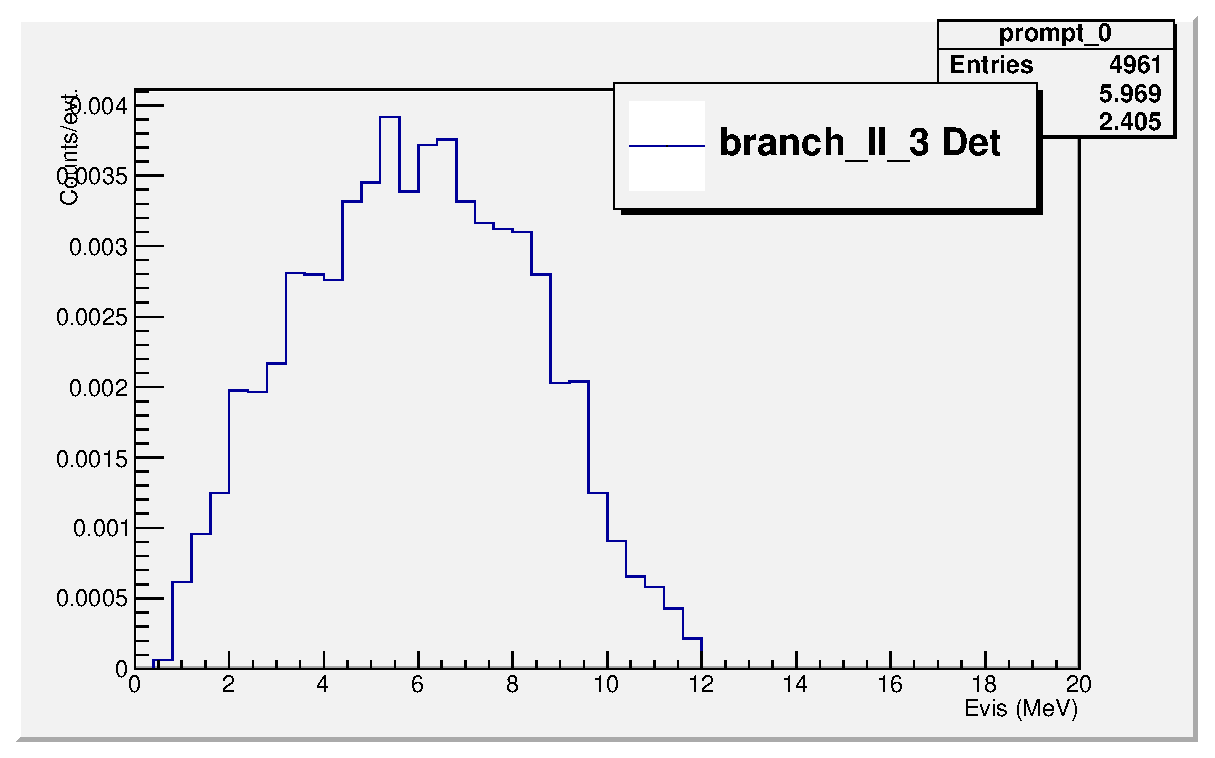
\includegraphics[width=60mm]{MC_Li_13.eps}&

    \includegraphics[width=60mm]{MC_Li_20.eps}\\

      \includegraphics[width=60mm]{MC_Li_21.eps}&

    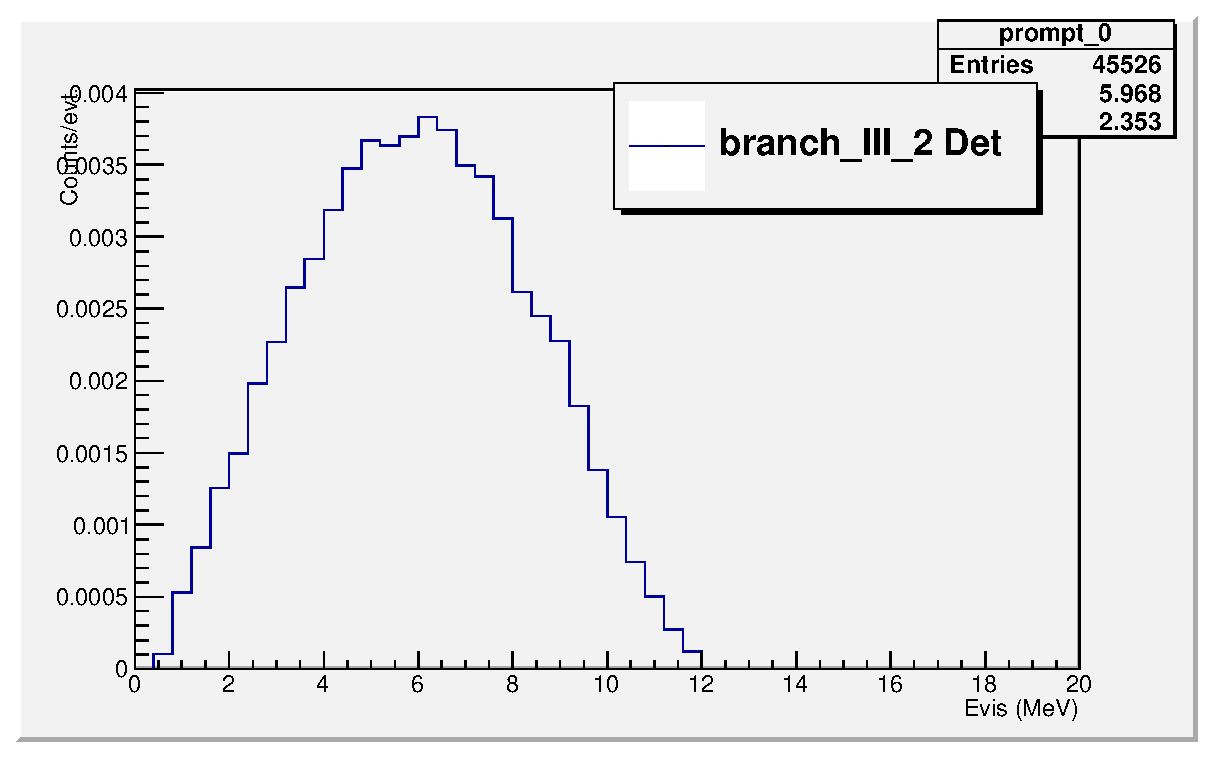
\includegraphics[width=60mm]{MC_Li_22.eps}\\
   
  \end{tabular}
\label{figur2}\caption{ Detector level energy distributions.}
\end{figure}




\section{Conclusions}
\label{section3}
Asoiuh siuhihosi soiu hskjd asoiuh siuhihosi soiu hskjd.  Asoiuh
siuhihosi soiu hskjd asoiuh siuhihosi soiu hskjd. Asoiuh siuhihosi
soiu hskjd asoiuh siuhihosi soiu hskjd. Asoiuh siuhihosi soiu hskjd
asoiuh siuhihosi soiu hskjd. Asoiuh siuhihosi soiu hskjd asoiuh
siuhihosi soiu hskjd. Asoiuh siuhihosi soiu hskjd asoiuh siuhihosi
soiu hskjd. Asoiuh siuhihosi soiu hskjd asoiuh siuhihosi soiu hskjd.


\acknowledgments

        TDDDDDDDDDDDDDDDDDDDDDDDDDDD


\bibliography{mybib}{}
\bibliographystyle{plain}

\end{document}
